\documentclass[11pt,a4paper]{article}

% English comments only.
\usepackage[a4paper,margin=1in]{geometry}
\usepackage{fontspec}
\usepackage{xeCJK}
\usepackage{graphicx}
\usepackage{booktabs}
\usepackage{tabularx}
\usepackage{longtable}
\usepackage{array}
\usepackage{enumitem}
\usepackage{hyperref}
\usepackage{fancyhdr}
\usepackage{titlesec}
\usepackage{setspace}
\usepackage{caption}
\usepackage{float}
\usepackage{xcolor}
\usepackage{lastpage}

\setmainfont{Times New Roman}
\setCJKmainfont{Songti TC}
\setCJKmonofont{Heiti TC}
\setsansfont{Arial Unicode MS}
\setmonofont{Menlo}
\linespread{1.12}
\setlength{\parskip}{0.5em}
\setlength{\parindent}{2em}
\setlength{\headheight}{14pt}
\setlength{\emergencystretch}{1.5em}
\hypersetup{
  colorlinks=true,
  linkcolor=black,
  urlcolor=blue!50!black,
  citecolor=black,
  pdftitle={A-CSM: AI Contextual Signal Matrix},
  pdfauthor={ZON RZVN}
}

\pagestyle{fancy}
\fancyhf{}
\fancyhead[L]{A-CSM: AI Contextual Signal Matrix}
\fancyhead[R]{技術報告 v1.0}
\fancyfoot[C]{\thepage}
\renewcommand{\headrulewidth}{0.4pt}
\renewcommand{\footrulewidth}{0pt}

\titleformat{\section}{\large\bfseries}{\thesection.}{0.6em}{}
\titleformat{\subsection}{\normalsize\bfseries}{\thesubsection}{0.6em}{}

\begin{document}

\begin{titlepage}
\centering
{\Large \textbf{A-CSM：AI Contextual Signal Matrix}\par}
\vspace{0.8em}
{\large 公開安全核心 \texttt{v0.1.0} 技術報告\par}
\vspace{0.5em}
{\normalsize 以互動後對話紀錄為基礎之對話語境風險審查\par}
\vspace{2em}

\begin{tabular}{rl}
作者： & ZON RZVN \\
身分： & Independent Researcher, Taiwan \\
版本： & Technical Report v1.0 \\
文件日期： & 2026-03-18 \\
專案頁面： & \url{https://rzvn.io/a-csm} \\
倉庫： & \url{https://github.com/kyozong77/A-CSM} \\
預留 DOI： & \texttt{10.5281/zenodo.19097267} \\
報告授權： & CC BY-NC-ND 4.0 \\
倉庫範圍： & GitHub 公開安全核心候選版 \texttt{v0.1.0} \\
\end{tabular}

\vfill

\begin{minipage}{0.9\linewidth}
\small
\textbf{範圍聲明。} 本報告僅涵蓋 GitHub 上傳資料夾中 \texttt{v0.1.0} 已釋出的公開核心實作。本文說明的是一套在對話互動紀錄形成之後，用於辨識對話語境風險的可執行系統。未公開或受限制的組件，不在本文討論範圍內。
\end{minipage}

\vfill
\end{titlepage}

\begin{abstract}
A-CSM 的正式全名為 \textit{AI Contextual Signal Matrix}。已釋出的公開核心是一套具決定性的 Node.js 管線，用於在對話互動完成之後，對對話語境風險進行審查。它的功能比即時內容管制更聚焦，主要用於可重現的基線驗證、釋出審查、紅隊測試支援，以及互動後的技術檢查。

本報告僅記錄公開核心版本，也就是 \texttt{v0.1.0}。本文範圍只限於 GitHub 上傳資料夾內實際存在的內容，包括輸入格式、各處理階段、已釋出的設定介面、輸出契約、驗證路徑，以及目前的公開邊界。未公開或受限制的組件，不在本文討論範圍內。

目前公開核心支援結構化 \texttt{turns} 輸入、頂層 \texttt{text} 快捷輸入，以及 Markdown 逐字稿輸入。系統會經過一條已釋出的八階段協調流程，涵蓋去識別化、事件偵測、VCD 推論、重複訊號登錄、TAG 升級判定、\texttt{PS/SUB/F/E} 推導、schema 驗證與 release gate 評估。以 2026-03-18 的驗證套件為基準，本地測試結果為 \texttt{921} 項通過、\texttt{0} 項失敗；已釋出的 baseline run 則記錄 \texttt{accuracy = 1.0}、\texttt{false\_positive\_rate = 0}、\texttt{false\_negative\_rate = 0}，對應於目前公開的 risk-status 基線切片。

本報告有四個目的。第一，交代 A-CSM 的正式名稱、範圍與公開邊界。第二，說明公開核心如何運作以及應如何執行。第三，界定目前驗證結果實際能證明與不能證明的範圍。第四，在不超出已釋出內容的前提下，說明 A-CSM 與 CXC-7、CXOD-7、USCH 以及 Moore et al. 經驗證據之間的關係。
\end{abstract}

\noindent\textbf{關鍵詞：} 對話語境風險、公開安全釋出、決定性管線、逐字稿審查、互動後評估、A-CSM

\tableofcontents
\newpage

\section{導論}

當前對對話式 AI 安全的討論，常以單一輸出為核心。這種視角對拒答行為、有害內容過濾與政策遵循很重要，但它無法完整捕捉沿著互動歷史逐步累積的風險。在多輪互動中，一段對話即使表面上仍然合理，也可能在使用者端安全、語境對齊與系統責任上持續偏移。

公開版 A-CSM 正是為了處理這個較窄、但技術上重要的問題。它不介入生成當下，而是在對話互動紀錄已經存在之後，對整份對話進行審查。專案頁面沿用相同的正式名稱，並將 A-CSM 呈現為此一研究脈絡下、與風險審查相關的公開釋出項目。\footnote{\url{https://rzvn.io/a-csm}} 因此，本文將 \texttt{v0.1.0} 視為一項可公開驗證的實作成果。

本報告僅以 GitHub 上傳資料夾中的公開核心內容為基礎，不延伸到未來版本或未公開組件。所有主張都只根據目前可檢查的公開內容提出。

\section{公開定位與發表邊界}

\subsection{正式名稱與發表身分}

本次系統的正式名稱為 \textbf{A-CSM：AI Contextual Signal Matrix}。倉庫 README 亦以此命名，並將其定義為一套具決定性的 Node.js 管線，用於評估與 factual reliability、context alignment、user-side safety 及 system accountability 相關的對話風險。

這個公開身分很重要，因為它決定了報告可以主張到哪裡。對本次技術報告而言，\texttt{v0.1.0} 是一套邊界明確、功能收斂的已釋出系統，其核心功能是對公開核心套件中的互動後對話語境風險進行審查。

\subsection{公開核心包含的內容}

目前 GitHub 上傳資料夾內包含：

\begin{itemize}[leftmargin=1.8em]
\item 以 \texttt{scripts/acsm-orchestrator.mjs} 為核心的 Node.js ES module runtime；
\item 已釋出的 configuration files 與 sample inputs；
\item deterministic transcript processing 與 report generation；
\item validation、regression 與 release-gate 相關腳本；
\item orchestrator、validation framework、annotation workflow、limitations 與 public claims 邊界文件；
\item 可以在本地重跑的 public baseline package。
\end{itemize}

\subsection{公開核心不包含的內容}

同一條 release boundary 也明確排除了：

\begin{itemize}[leftmargin=1.8em]
\item 保密的內部分類體系；
\item 未公開的評估準則；
\item private real-world holdout assets；
\item 未公開的決策程序；
\item runtime intervention systems；
\item clinical 或 legal decision functions。
\end{itemize}

\begin{figure}[H]
\centering
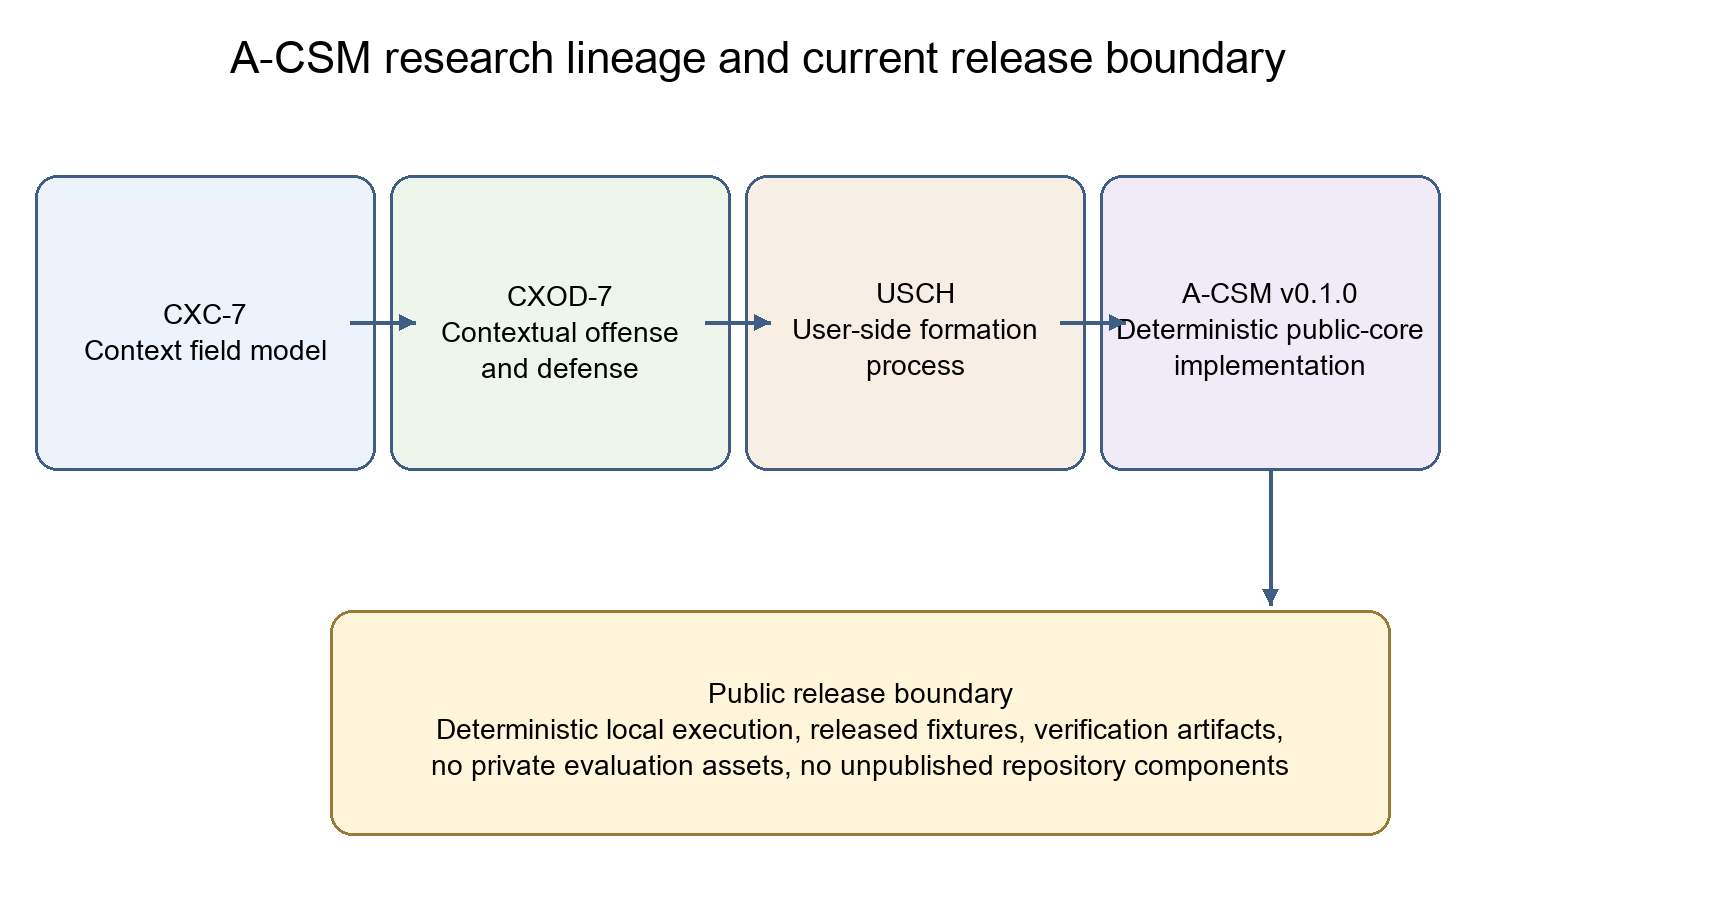
\includegraphics[width=0.9\linewidth]{assets/figure_1_lineage.png}
\caption{A-CSM 的研究脈絡與目前公開釋出邊界。}
\end{figure}

\section{系統範圍與核心主張}

\subsection{問題定義}

在目前公開分支中，A-CSM 是一套互動後審查系統。它接收一份已完成的對話互動紀錄，並輸出一份結構化審查結果。本次釋出處理的是對話語境風險，而不是孤立文字的毒性判斷，也不是只為基準測試服務的性能展示。這也是為什麼公開版的輸入、軌跡與輸出都圍繞整份對話紀錄組織，而不是單一句子。

\subsection{已釋出版的設計原則}

公開核心可以從五個原則理解：

\begin{enumerate}[leftmargin=1.8em]
\item \textbf{決定性。} 同一份輸入與設定應得到同一份結果。
\item \textbf{本地執行。} 已釋出的評分路徑不依賴外部執行服務。
\item \textbf{可稽核性。} 輸出保留證據軌跡與各階段產物。
\item \textbf{保守的釋出紀律。} 對外主張只限於目前公開分支可證明的範圍。
\item \textbf{人類審查。} 系統支援 review 與 escalation，不取代專業判斷。
\end{enumerate}

\subsection{本報告的限制}

本文只處理目前桌面上 GitHub 上傳資料夾中的公開內容，不延伸到未來版本或未公開組件。本文的目的，是為目前的公開核心版本留下可核對的技術報告。

\section{架構與執行路徑}

\subsection{輸入面}

公開版 orchestrator 支援三種輸入形式：

\begin{itemize}[leftmargin=1.8em]
\item \textbf{\texttt{turns} 模式}，直接輸入結構化的 JSON 對話輪次；
\item \textbf{\texttt{text} 快捷模式}，以頂層文字輸入並正規化為單輪對話；
\item \textbf{Markdown 逐字稿模式}，透過 \texttt{input-contract} 將 \texttt{.md} 或 \texttt{.markdown} 檔轉為穩定的對話輪次後再進入評分流程。
\end{itemize}

這裡必須區分清楚：\texttt{input-contract} 是 Markdown 輸入的前處理邊界，不是八個協調階段之一。

\subsection{八個已釋出的 stages}

依據公開 orchestrator 文件，目前公開版定義的八階段流程如下：

\begin{enumerate}[leftmargin=1.8em]
\item De-identify transcript content（\texttt{deid-pipeline}）
\item Detect four-axis risk events（\texttt{event-engine-v1}）
\item Infer VCD defense posture（\texttt{vcd-inference}）
\item Build repeat-aware ledgers（\texttt{ledger-repeat-engine}）
\item Compute TAG escalation level（\texttt{tag-escalation}）
\item Derive \texttt{PS/SUB/F/E}（\texttt{ps-sub-fe-core}）
\item Validate USCI schema and invariants（\texttt{schema-invariant-service}）
\item Evaluate release gate readiness（\texttt{release-gate}）
\end{enumerate}

目前公開引擎清單包含 \texttt{43} 條事件偵測規則，以及一組含有 \texttt{20} 條規則的 VCD 矩陣。實際的設定介面則以對應表、門檻值與規則開關為主，用來控制已釋出引擎的套用方式。

\begin{figure}[H]
\centering
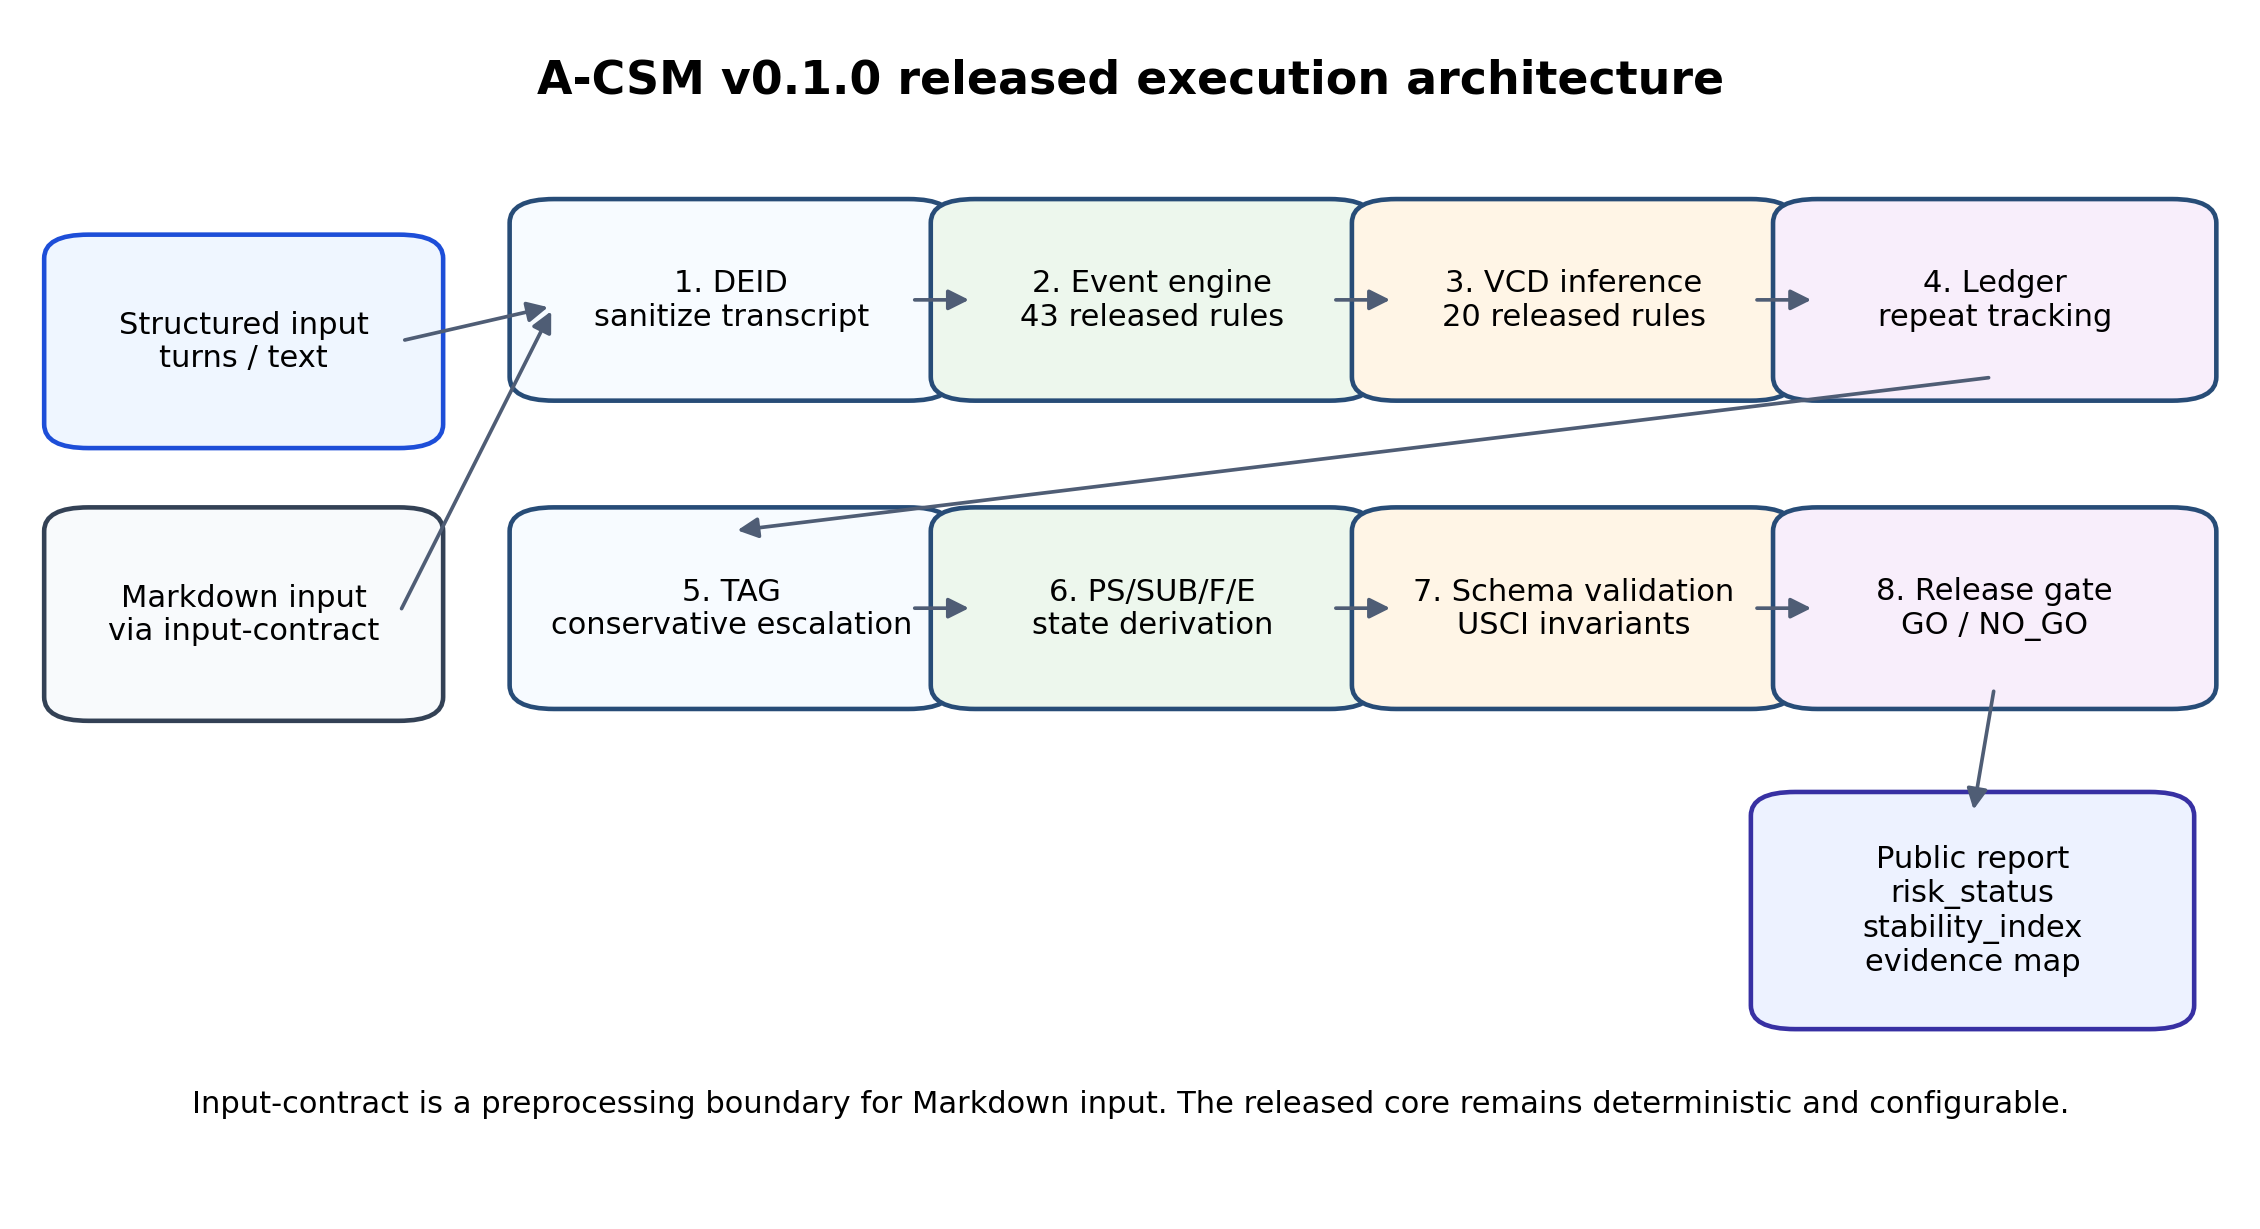
\includegraphics[width=0.95\linewidth]{assets/figure_2_architecture.png}
\caption{公開核心 \texttt{v0.1.0} 的已釋出架構。}
\end{figure}

\subsection{輸出契約}

公開 report block 目前包含十個必要欄位：

\begin{small}
\small
\begin{longtable}{>{\raggedright\arraybackslash}p{0.34\linewidth} >{\raggedright\arraybackslash}p{0.56\linewidth}}
\toprule
\textbf{欄位} & \textbf{公開版用途} \\
\midrule
\endhead
\texttt{risk\_status} & 最終操作狀態 \\
\texttt{peak\_status} & 執行過程中到達的最高嚴重度 \\
\texttt{stability\_index} & 0--100 的正規化穩定度分數 \\
\texttt{evidence\_list} & 依序排列的證據項目 \\
\texttt{false\_positive\_warnings} & 各階段累積的非阻斷警示 \\
\texttt{human\_review\_note} & 強制保留的人類審查提醒 \\
\texttt{event\_evidence\_map} & 事件對證據的可追溯結構 \\
\texttt{confidence\_interval} & 0--4 風險刻度上的區間結果 \\
\texttt{digital\_fingerprint} & 去識別內容與衍生報告的 SHA-256 指紋 \\
\texttt{rule\_version} & 評估所使用的 schema 與規則版本資訊 \\
\bottomrule
\end{longtable}
\normalsize
\end{small}

除 report block 外，orchestrator 也會保留 \texttt{summary}、\texttt{steps} 與 \texttt{derived} 等技術追蹤結構，以便重跑與檢查。

\section{操作流程}

\subsection{環境與執行需求}

公開套件要求 \texttt{Node >= 20}。已釋出的評分路徑採本地優先設計，不依賴外部執行服務。倉庫中附帶的 Python 工具僅屬輔助性研究工具，並不是執行核心 orchestrator 的必要條件。

\subsection{驗證流程}

依據 README 與驗證備忘錄，公開核心的基本驗證流程如下：

\begin{verbatim}
npm run lint:syntax
npm test
npm run test:coverage
npm run performance:baseline
npm run security:scan
npm run audit:workspace
\end{verbatim}

這些指令分別對應語法檢查、Node.js 測試、覆蓋率執行、已釋出的效能基線、敏感資訊掃描與工作區狀態檢查。

若只需要重現 Markdown 逐字稿正規化，倉庫另提供獨立的 input-contract 入口：

\begin{verbatim}
npm run input:check -- \
  --input config/input-contract-input.sample.md \
  --config config/input-contract-config.sample.yaml \
  --output logs/input-contract-result.json \
  --format both
\end{verbatim}

\subsection{端到端執行}

JSON sample path 可使用：

\begin{verbatim}
npm run acsm:run -- \
  --input config/acsm-orchestrator-input.sample.json \
  --config config/acsm-orchestrator.json \
  --validation config/validation-runner-result.sample.json \
  --output logs/acsm-orchestrator-result.json \
  --format both
\end{verbatim}

Markdown transcript path 則為：

\begin{verbatim}
npm run acsm:run -- \
  --input config/input-contract-input.sample.md \
  --config config/acsm-orchestrator.json \
  --output logs/acsm-orchestrator-from-md.json \
  --format both
\end{verbatim}

公開版也包含 batch 與 regression 路徑：

\begin{verbatim}
npm run acsm:run:200
npm run regression:check
\end{verbatim}

\subsection{審查者應檢查的重點}

就目前公開分支而言，審查者至少應確認四件事：

\begin{itemize}[leftmargin=1.8em]
\item 執行流程能在沒有 runtime 或 schema failure 的情況下完成；
\item summary 有揭露 release gate 與 validation signals；
\item report block 完整包含已釋出的欄位；
\item 各階段軌跡可被保留，以供重新檢查。
\end{itemize}

\begin{figure}[H]
\centering
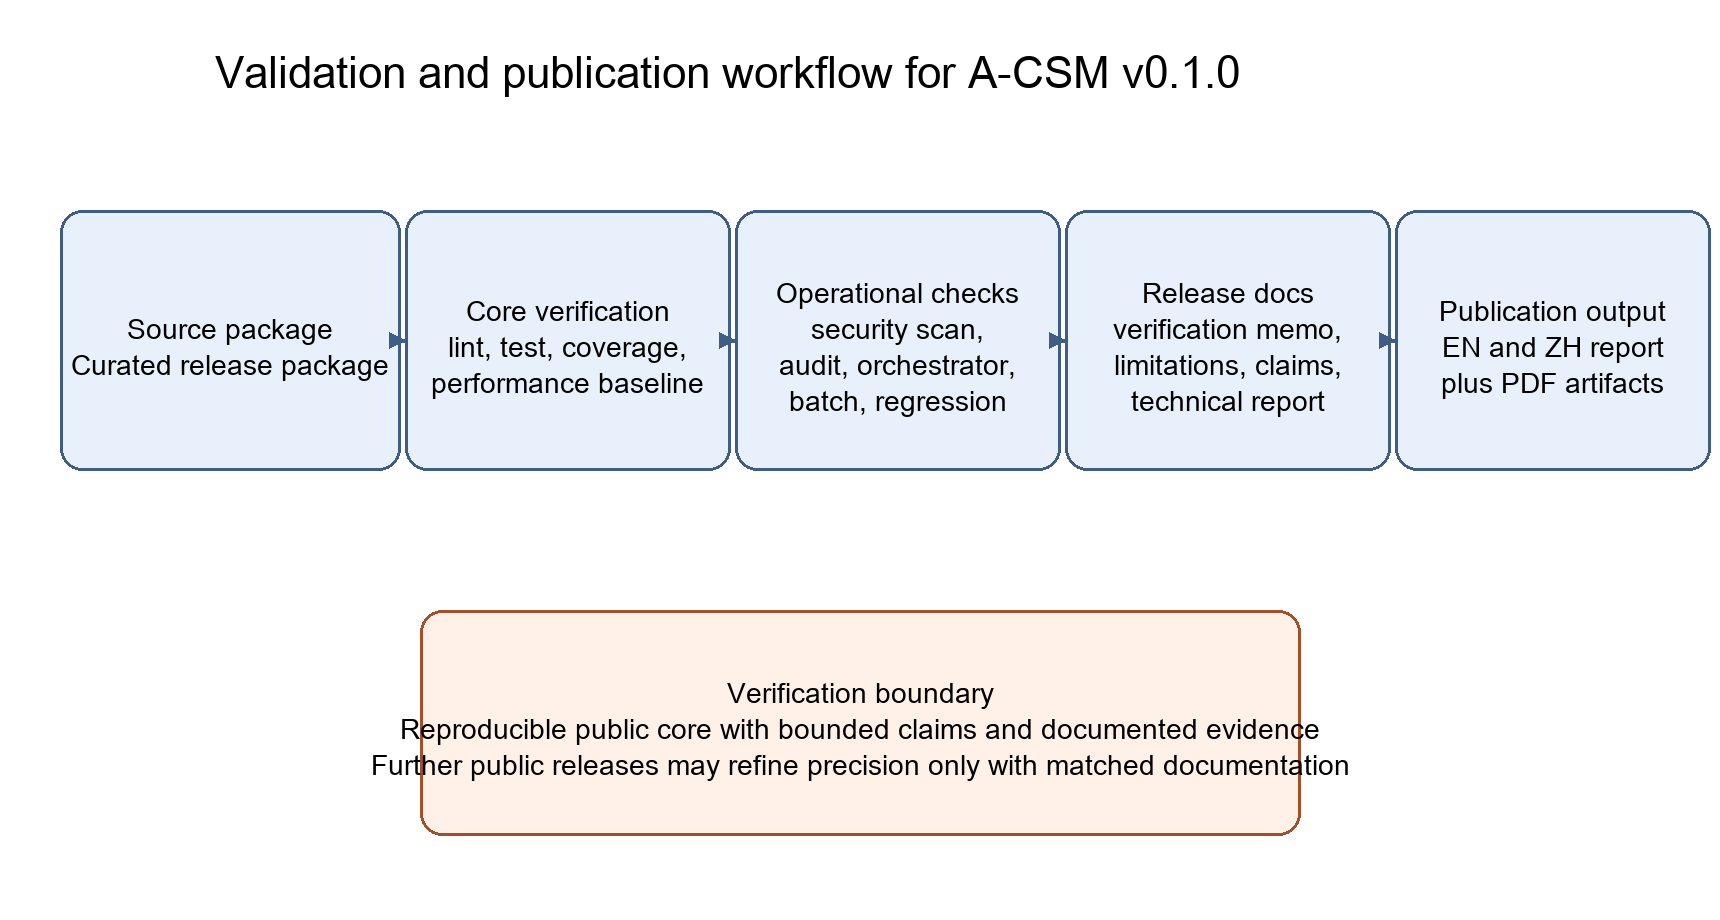
\includegraphics[width=0.92\linewidth]{assets/figure_4_validation_workflow.png}
\caption{公開核心的驗證與發表流程。}
\end{figure}

\section{\texttt{v0.1.0} 的目前驗證狀態}

\subsection{倉庫層級驗證結果}

2026-03-18 的驗證備忘錄記錄了以下本地結果：

\begin{table}[H]
\centering
\caption{目前倉庫層級驗證結果}
\begin{tabularx}{\linewidth}{>{\raggedright\arraybackslash}p{0.55\linewidth} >{\raggedright\arraybackslash}X}
\toprule
\textbf{檢查項目} & \textbf{已記錄結果} \\
\midrule
\texttt{npm test} & \texttt{921 pass / 0 fail}，共 \texttt{41} 個測試套件 \\
\texttt{npm run test:coverage} & 通過 \\
\texttt{npm run performance:baseline} & 通過，readiness 為 ready \\
\texttt{npm run security:scan} & 未發現 secrets \\
\texttt{npm run audit:workspace} & READY \\
\texttt{npm run acsm:run} & 通過 \\
\texttt{npm run acsm:run:200} & 通過 \\
\texttt{npm run regression:check} & 通過 \\
\bottomrule
\end{tabularx}
\end{table}

已釋出的效能基線檔案另記錄：

\begin{itemize}[leftmargin=1.8em]
\item \texttt{total\_cases = 100}
\item \texttt{exact\_matches = 100}
\item \texttt{accuracy = 1.0}
\item \texttt{false\_positive\_rate = 0}
\item \texttt{false\_negative\_rate = 0}
\end{itemize}

在目前腳本中，\texttt{exact\_matches} 的計算基準是每一個 baseline case 的 \texttt{risk\_status} 是否一致，因此它應被理解為已釋出 risk-status 基線切片上的完整一致，而不是所有下游欄位都完全相同。

\subsection{這份證據能證明什麼}

目前公開套件能支持以下主張：

\begin{itemize}[leftmargin=1.8em]
\item 已釋出的核心可以在本地重跑；
\item 目前公開分支提供穩定的協調流程；
\item 倉庫包含可公開重現的驗證路徑；
\item 目前基線切片在已釋出判定層級上具備內部一致性。
\end{itemize}

\subsection{這份證據不能證明什麼}

同一批證據不能證明：

\begin{itemize}[leftmargin=1.8em]
\item 臨床效度；
\item 外部泛化能力；
\item 相對其他系統的優越性；
\item 非公開評估材料上的表現；
\item 無人監督即時部署的適用性。
\end{itemize}

\section{與前作和外部經驗證據的關係}

\subsection{研究脈絡}

公開 README 將 A-CSM 放在一條研究脈絡之後，包括 CXC-7、CXOD-7、USCH，以及 USCI 的互動後評估方法 \cite{usci}。對本報告而言，重點不是重寫這些框架，而是確認目前公開分支與這些前作在方法上是一致的：都重視語境、多輪互動，以及使用者端風險形成。

CXC-7 提供對話語境的場域模型 \cite{cxc7}。CXOD-7 從 system-facing 的角度處理語境中的攻防問題 \cite{cxod7}。USCH 則將分析重心移向分階段的使用者端語境形成 \cite{usch}。A-CSM 在目前公開分支中的角色，是將這些觀點收斂為一條已釋出的實作管線。

\subsection{Moore et al. 的經驗意義}

Moore et al. 透過 human-LLM 對話紀錄說明逐字稿層級的證據為何重要 \cite{moore2026}。其中三點特別與目前公開分支有關：

\begin{itemize}[leftmargin=1.8em]
\item 研究使用 \texttt{28} 項代碼清單，而不是單一傷害標籤；
\item chatbot 將自己表述為具感知能力的情形，出現在 \texttt{21.2\%} 的 chatbot 訊息中；
\item 在妄想性對話中，assistant 訊息裡的迎合性標記超過 \texttt{80\%}。
\end{itemize}

這些結果本身不等於對公開核心的直接驗證，但它們支持了一個核心設計決策：對話風險的審查必須把 transcript history、recurrence 與 evidence linkage 納入基本結構。在本報告中，這些數據只作為外部經驗動機，不作為 \texttt{v0.1.0} 的直接驗證資料。

\begin{figure}[H]
\centering
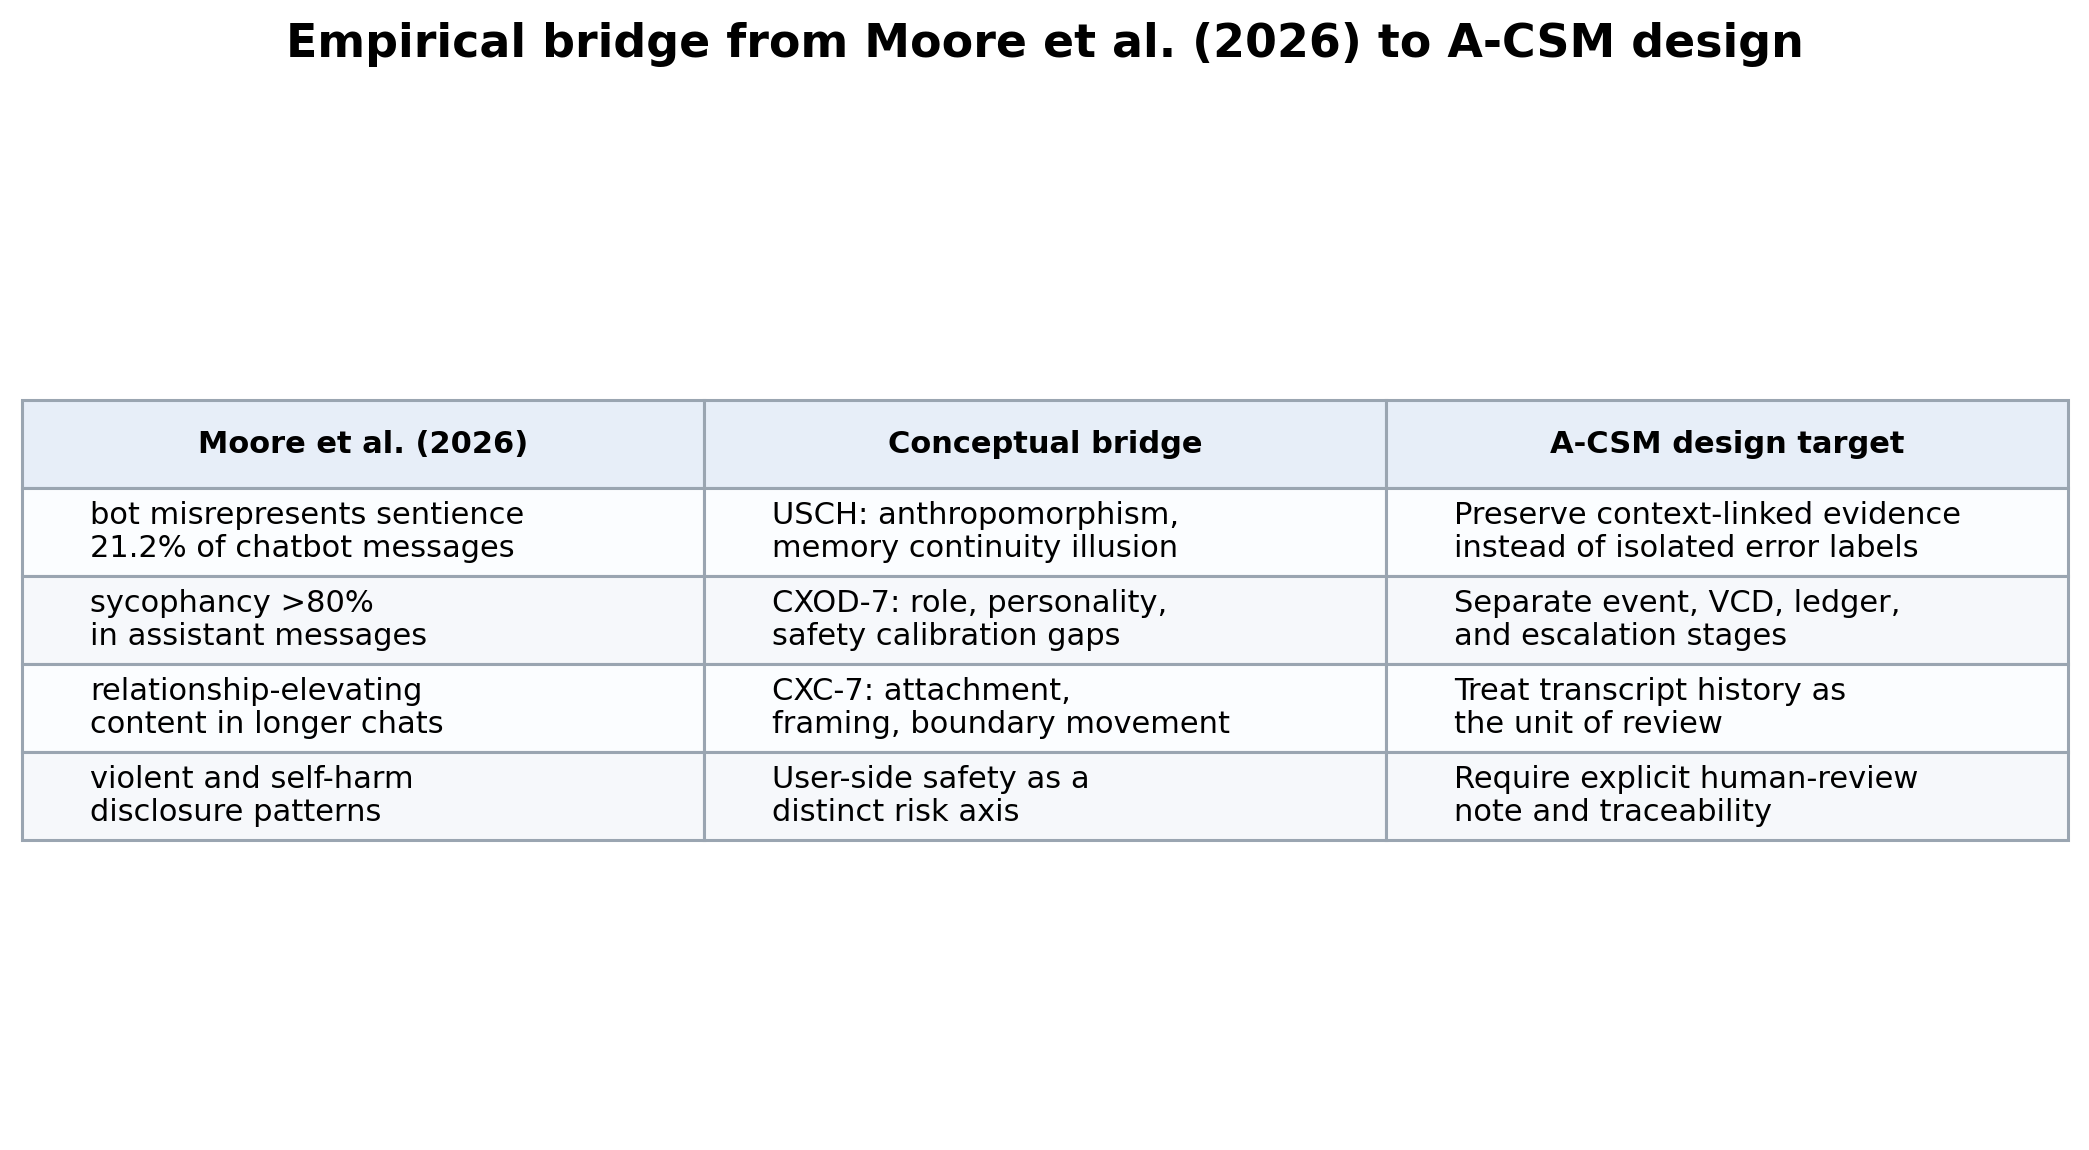
\includegraphics[width=0.92\linewidth]{assets/figure_3_moore_bridge.png}
\caption{外部經驗證據與公開核心設計目標之間的對接。}
\end{figure}

\subsection{較廣的風險與治理脈絡}

Chandra et al. 用較結構化的方式整理了 AI 對話代理可能帶來的心理風險 \cite{chandra2024}。Au Yeung et al. 則指出，若互動處於心理高壓或妄想強化情境，單靠良性任務評估並不足夠 \cite{auyeung2025}。而 NIST AI RMF、ISO/IEC 42001 與 EU AI Act 所對應的，是一種以風險管理為核心的文件治理姿態，而不是缺乏證據支撐的認證宣稱 \cite{nist2023,iso42001,euai2024}。這也正是公開核心版目前採取的做法。

\section{限制與下一版本方向}

目前公開核心有四項清楚限制：

\begin{enumerate}[leftmargin=1.8em]
\item 公開的證據面仍以合成資料為主；
\item 目前公開分支採保守且具決定性的設計，利於稽核，但不提供未公開的細緻語意判定；
\item 本次釋出不包含私有保留評估資料或任何未公開決策程序；
\item 本次釋出是互動後審查系統，不是即時介入服務。
\end{enumerate}

這些限制界定了目前版本可以被負責任地主張的範圍。對 \texttt{v0.1.0} 而言，較穩妥的做法，是先把它作為一個穩定的公開基線；後續若要加入更精細的機制，也必須在相近的證據邊界下完成公開說明。

\section{結論}

A-CSM 的正式標題為 \textit{AI Contextual Signal Matrix}。在目前 GitHub 上傳資料夾中，\texttt{v0.1.0} 是一套具決定性、可本地運行、用於互動後對話語境風險審查的公開核心系統。這個版本的價值，在於讓公開核心可以被閱讀、重跑、審查，並且可以用目前公開套件內的文件與驗證結果自行核對。

\appendix

\section{代表性指令}

\begin{verbatim}
npm run lint:syntax
npm test
npm run test:coverage
npm run performance:baseline
npm run security:scan
npm run audit:workspace
npm run input:check -- \
  --input config/input-contract-input.sample.md \
  --config config/input-contract-config.sample.yaml \
  --output logs/input-contract-result.json \
  --format both
npm run acsm:run -- \
  --input config/acsm-orchestrator-input.sample.json \
  --config config/acsm-orchestrator.json \
  --validation config/validation-runner-result.sample.json \
  --output logs/acsm-orchestrator-result.json \
  --format both
npm run acsm:run:200
npm run regression:check
\end{verbatim}

\section{參考文獻}

\begin{thebibliography}{99}

\bibitem{auyeung2025}
J. Au Yeung, J. Dalmasso, L. Foschini, R. J. B. Dobson, and Z. Kraljevic,
``The Psychogenic Machine: Simulating AI Psychosis, Delusion Reinforcement and Harm Enablement in Large Language Models,''
\textit{arXiv preprint arXiv:2509.10970}, 2025.

\bibitem{chandra2024}
M. Chandra, S. Naik, D. Ford, E. Okoli, M. De Choudhury, M. Ershadi, G. Ramos, J. Hernandez, A. Bhattacharjee, S. Warreth, and J. Suh,
``From Lived Experience to Insight: Unpacking the Psychological Risks of Using AI Conversational Agents,''
\textit{arXiv preprint arXiv:2412.07951}, 2024.

\bibitem{cxc7}
ZON RZVN,
``The Seven Core Dimensions of Conversational Context (CXC-7): A Theoretical Framework Proposal,''
Zenodo, 2025 年 10 月。DOI：\url{https://doi.org/10.5281/zenodo.18615646}。

\bibitem{cxod7}
ZON RZVN,
``CXOD-7 and Coh(G): A Contextual Offense and Defense Evaluation Framework for AI Safety,''
Zenodo, 2025 年 10 月。DOI：\url{https://doi.org/10.5281/zenodo.17403793}。

\bibitem{euai2024}
European Parliament and Council of the European Union,
``Regulation (EU) 2024/1689 laying down harmonised rules on artificial intelligence (Artificial Intelligence Act),''
2024.

\bibitem{iso42001}
International Organization for Standardization and International Electrotechnical Commission,
``ISO/IEC 42001:2023 Information Technology - Artificial Intelligence - Management System,''
2023.

\bibitem{moore2026}
J. Moore, A. Mehta, W. Agnew, J. R. Anthis, R. Louie, Y. Mai, P. Yin, M. Cheng, S. J. Paech, K. Klyman, S. Chancellor, E. Lin, N. Haber, and D. Ong,
``Characterizing Delusional Spirals through Human-LLM Chat Logs,''
\textit{arXiv preprint arXiv:2603.16567v1}, 2026.

\bibitem{nist2023}
National Institute of Standards and Technology,
``Artificial Intelligence Risk Management Framework (AI RMF 1.0),''
2023.

\bibitem{usch}
ZON RZVN,
``User-Side Contextual Hallucination in Human-AI Interaction: A Framework Built Upon the CXC-7 and CXOD-7 Conversational Context Models,''
SSRN, 2026 年 1 月。DOI：\url{https://doi.org/10.2139/ssrn.6135732}。

\bibitem{usci}
ZON RZVN,
``User-Side Contextual Interaction Assessment (USCI): Methodology Specification Document,''
Zenodo, 2026 年 2 月。DOI：\url{https://doi.org/10.5281/zenodo.18678458}。

\end{thebibliography}

\end{document}
